\documentclass[10pt,twoside]{article}

\usepackage[paperwidth=8.5in, paperheight=11in, margin=1in]{geometry}
\usepackage{booktabs}
\usepackage{longtable}
\usepackage{graphicx}
\usepackage[export]{adjustbox}
\usepackage{array}
\usepackage{float}
\usepackage{caption}
\captionsetup[table]{skip=10pt}
\renewcommand{\thepage}{S-\arabic{page}}
%\fancyfoot[RO,LE]{S-\thepage}

\newcolumntype{L}[1]{>{\raggedright\let\newline\\\arraybackslash\hspace{0pt}}p{#1}}
% define "struts", as suggested by Claudio Beccari in
%    a piece in TeX and TUG News, Vol. 2, 1993.
\newcommand\Tstrut{\rule{0pt}{2.6ex}}         % = `top' strut
\newcommand\Bstrut{\rule[-0.9ex]{0pt}{0pt}}   % = `bottom' strut

% \renewcommand{\familydefault}{\sfdefault}
\usepackage{fontspec}
\setmainfont{Times New Roman}
\setlength\parindent{0pt}

\renewcommand{\thefigure}{S-\arabic{figure}}
\renewcommand{\thetable}{S-\arabic{table}}

\newcommand{\footremember}[2]{%
  \footnote{#2}
  \newcounter{#1}
  \setcounter{#1}{\value{footnote}}%
}
\newcommand{\footrecall}[1]{%
  \footnotemark[\value{#1}]%
}
\title{Analysing the structure of pathways and its influence on the interpretation of biomedical proteomics datasets}
\author{Bram Burger%
  \footremember{CBU}{Computational Biology Unit (CBU), Department of Informatics, University of Bergen, 5020 Bergen, Norway.}
  \footremember{PROBE}{Proteomics Unit (PROBE), Department of Biomedicine, University of Bergen, 5020 Bergen, Norway.}%
  \and Luis Francisco Hern\'andez S\'anchez%
  \footremember{KGJ}{KG Jebsen Center for Diabetes Research, Department of Clinical Science, University of Bergen, 5020 Bergen, Norway.}
  \footremember{CMGMM}{Center for Medical Genetics and Molecular Medicine, Haukeland University Hospital, 5020 Bergen, Norway.}%
  \and Ragnhild Reehorst Lereim%
  \footrecall{CBU}
  \footrecall{PROBE}%
  \and Harald Barsnes%
  \footrecall{CBU}
  \footrecall{PROBE}
  \footremember{senior}{Senior author.}%
  \and Marc Vaudel%
  \footrecall{KGJ}
  \footrecall{CMGMM}
  \footrecall{senior}
  \footremember{correspondence}{To whom correspondence should be addressed: email: marc.vaudel@uib.no. Phone: +47 55 97 12 63 Postal address: Postboks 7804, 5020 Bergen, Norway}%
}
\date{}

\begin{document}
\maketitle
\tableofcontents
\listoffigures
\listoftables
\clearpage
\section{Supplementary methods}
Integration and Radiality were first decsribed in Valente and Foreman (1998).
The distance from node $j$ to node $k$ is the shortest path between these two, which is given by $d(j, k)$.
If there is no path from node $j$ to node $k$, this is defined as infinite.
Notice that, as we have a directed network, $d(j, k)$ is not necessarily the same as $d(k, j)$ and that there might be a path from $j$ to $k$ even if there is not a path the other way.
If we calculate the shortest path for each pair of nodes, the diameter of the network $D(G)$ is the longest of these shortest paths ignoring the ones of infinite length.
While the shortest path from node $j$ to node $k$ is given by $d(j, k)$, the inverse of this is defined as $RD(j,k) = D(G) + 1 - d(j, k)$: the diameter of the network plus one, minus the distance from node $j$ to node $k$.
If there is no path from $j$ to $k$ $RD(j,k)$ is defined as 0.
The total number of nodes in the network is $N$.

The Integration of node $k$ is then calculated as
\[ I(k) = \frac{\sum_{j \neq k}RD(j,k)}{D(G)(N-1)} \]
Similarly, the Radiality of node $k$ is then calculated as
\[ R(k) = \frac{\sum_{j \neq k}RD(k,j)}{D(G)(N-1)} \]

\clearpage

\begin{figure}
  \centering
  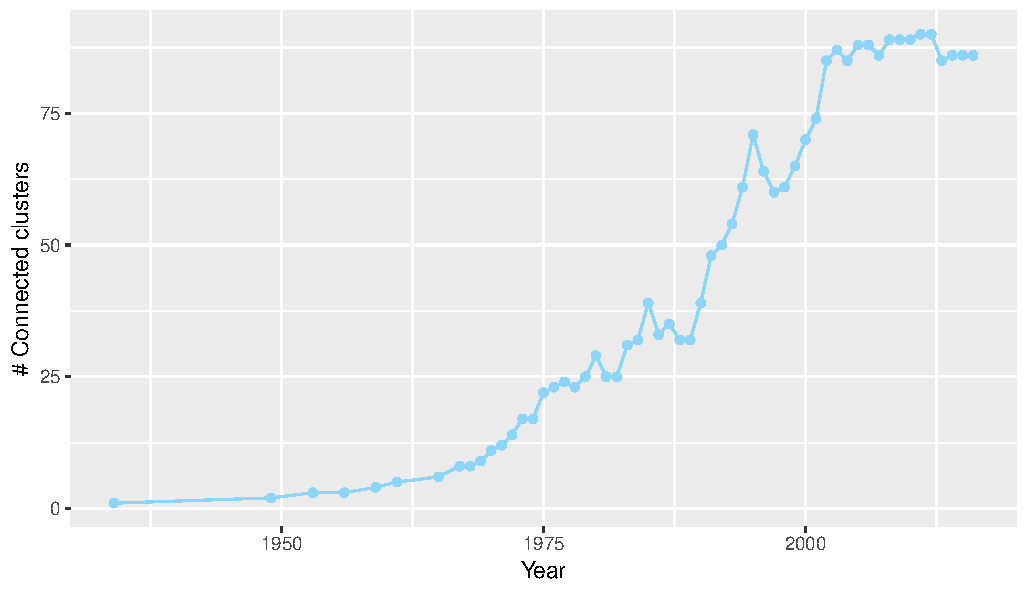
\includegraphics[width=0.9\textwidth]{../S1/FigureS1.pdf}
  \caption[Number of connected components per year]{Number of connected components per year.}
  \label{fig:s1}
\end{figure}

\begin{figure}
  \centering
  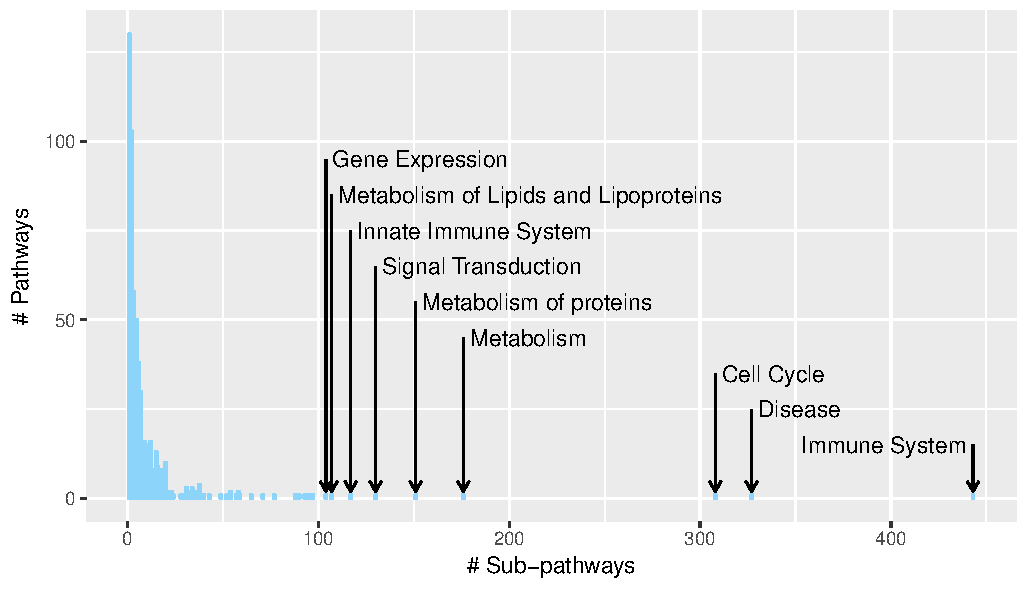
\includegraphics[width=0.9\textwidth]{../S2/FigureS2.pdf}
  \caption[Distribution of the number of sub-pathways for all
    pathways]{Distribution of the number of sub-pathways for all
    pathways. There are 2051 pathways annotated in total. Most
    pathways (1397) do not contain any sub-pathways. Of the remaining
    654, most contain few sub-pathways. The nine pathways with more
    than 100 sub-pathways are annotated in the plot. Innate Immune
    System is a sub-pathway of Immune System, Metabolism of Lipids and
    Lipoproteins is a sub-pathway of Metabolism, the other pathways
    are all top-level pathways.}
  \label{fig:s2}
\end{figure}

\begin{figure}
  \centering
  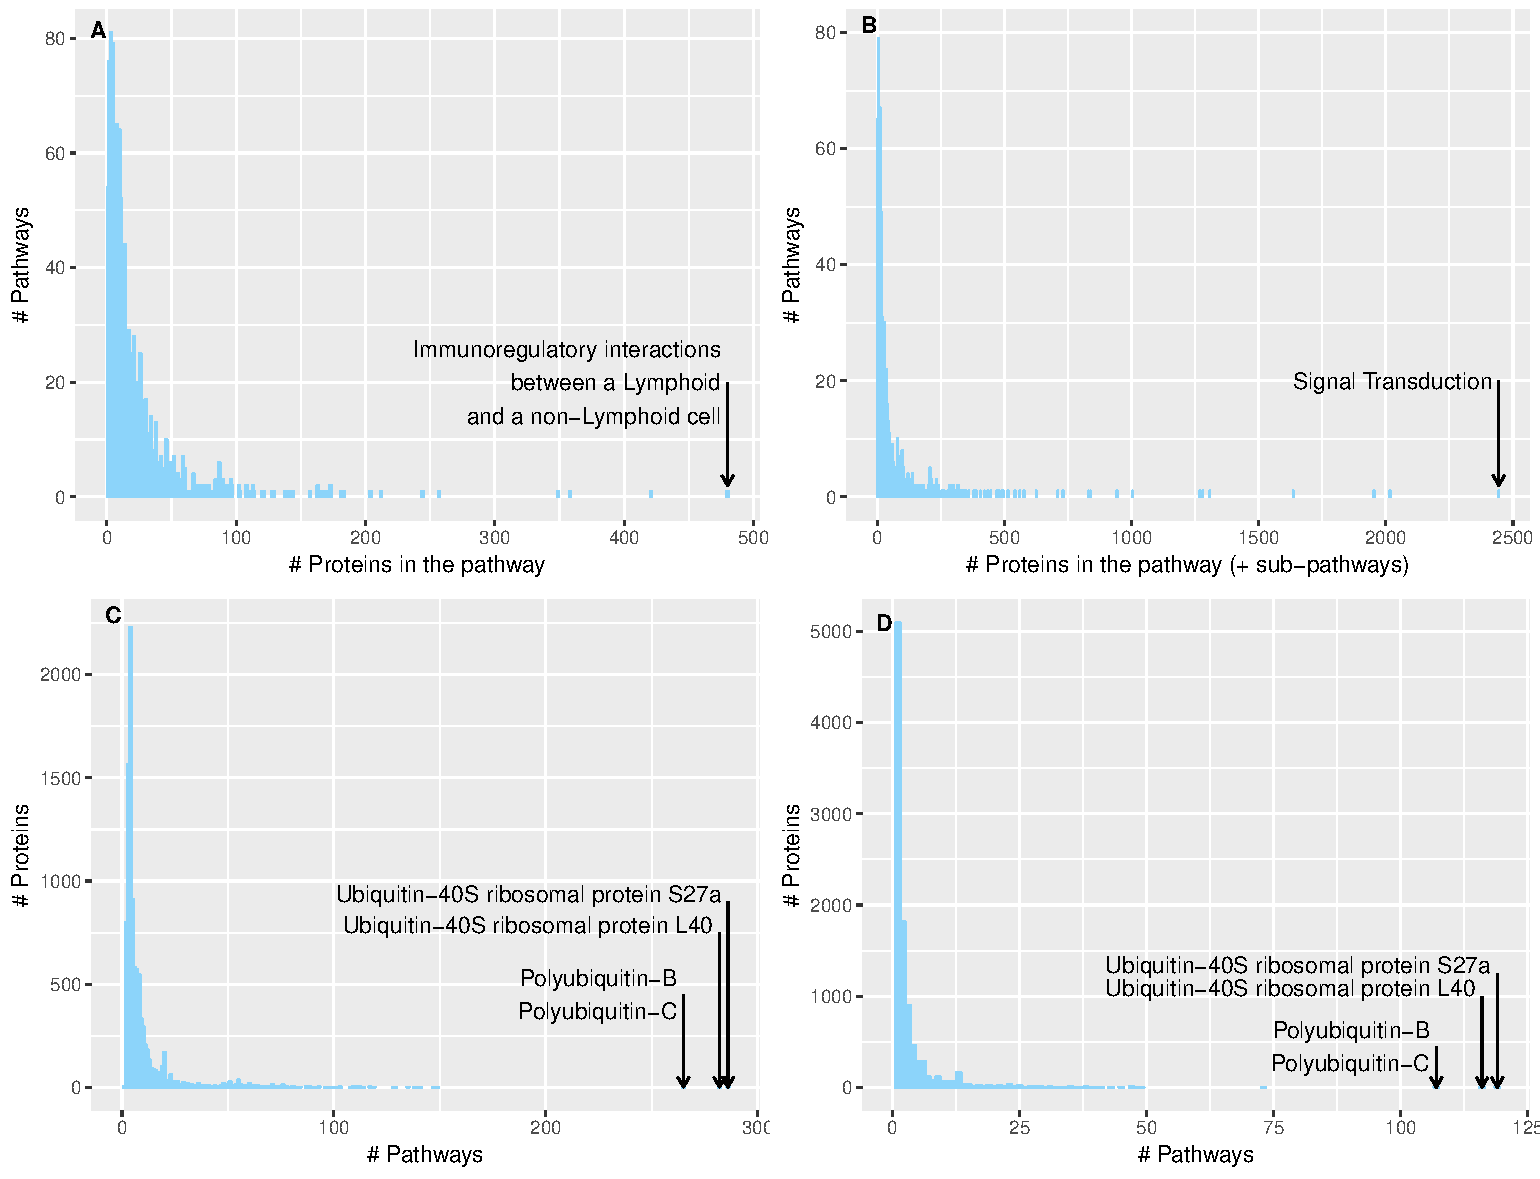
\includegraphics[width=0.9\textwidth]{../S3/FigureS3.pdf}
  \caption[Number of proteins per pathway and vice versa]{Number of proteins per pathway and vice versa. A) Number of
    proteins directly occurring in each pathway. B) Number of proteins
    occurring in each pathway, including the proteins occurring in
    sub-pathways. C) Number of pathways a protein occurs in, including
    the pathways where the protein occurs in a sub-pathway. D) Number
    of pathways a protein directly occurs in.}
  \label{fig:s3}
\end{figure}

\begin{figure}
  \centering
  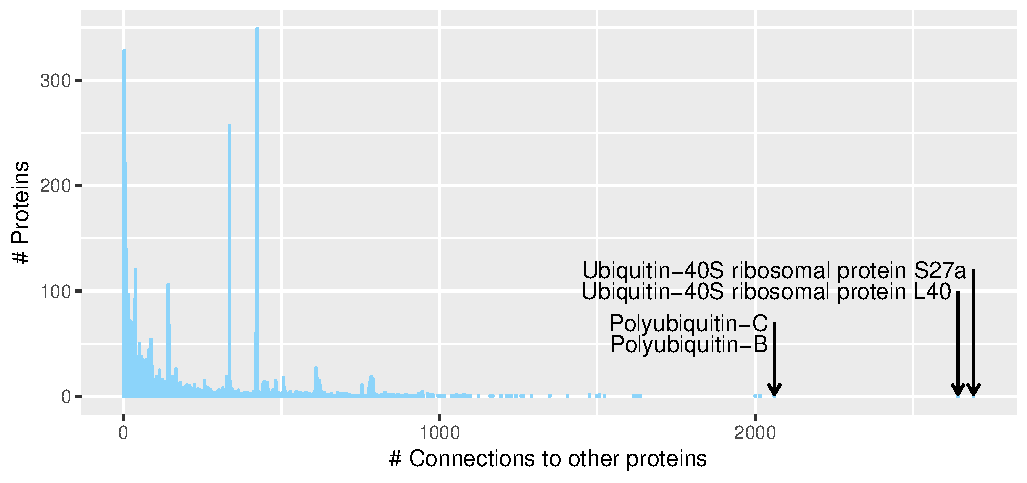
\includegraphics[width=0.9\textwidth]{../S4/FigureS4.pdf}
  \caption[Distribution of the number of connections for each protein]{Distribution of the number of connections for each protein.
    The two big spikes around 400 connections are mainly olfactory
    receptors and zinc fingers. 
  }
  \label{fig:s4}
\end{figure}

% \begin{figure}
%   \centering
%   \includegraphics[width=\textwidth]{../S5/FigureS5.pdf}
%   \caption{Protein network coloured by node type. Node types
%     consistent with the classification using radiality and
%     integration. Red: isolated proteins; green: proteins in the main
%     cluster; blue: start of chain proteins; purple: end of chain
%     proteins.}
%   \label{fig:s5}
% \end{figure}

\begin{figure}
  \centering
  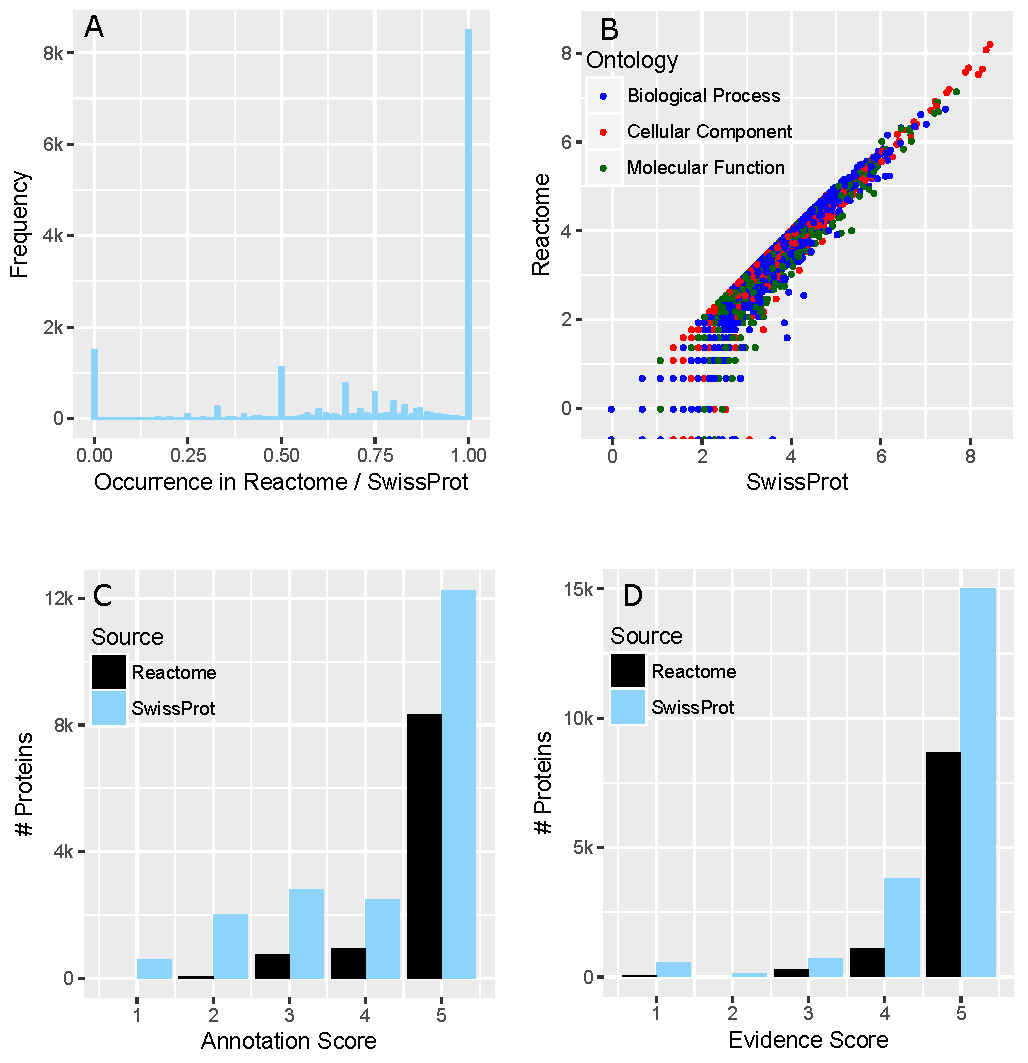
\includegraphics[width=\textwidth]{../S6/FigureS6.pdf}
  \caption[Potential biases in the curation process]{Potential biases in the curation process. Relative
    occurrence of GO terms (A and B) or protein annotations (C and D)
    in Reactome vs. SwissProt. A) The number of GO terms that occur
    with the relative amount indicated on the x-axis (bins of
    0.01). B) Each point indicates one GO term. The axes are
    log-scale, and terms not included in Reactome are plotted at the
    bottom of the plot. Red: Cellular Component; green: Molecular
    Function; blue: Biological Process. C) Distributions of annotation
    and D) evidence scores of proteins in SwissProt and
    Reactome. Higher scores indicate more annotation and better
    evidence. Reactome contains only about half of the proteins in
    SwissProt, hence the much lower bars in general for Reactome.}
  \label{fig:s6}
\end{figure}

\clearpage

\begin{table}[H]
  \centering
  \caption[The number of pathways a sub-pathway directly participates in]{The number of pathways a sub-pathway directly participates in. Only those sub-pathways that are directly part of more than two pathways are shown.}
  \begin{tabular}{lr}
    \toprule
    Pathway Name&	Parents\\\midrule
    RAF/MAP kinase cascade&	20\\
    PIP3 activates AKT signaling&	9\\
    DAG and IP3 signaling&	5\\
    TAK1 activates NFkB by phosphorylation and activation of IKKs complex&	4\\
    MAP kinase activation in TLR cascade&	4\\
    Spry regulation of FGF signaling&	4\\
    MyD88:Mal cascade initiated on plasma membrane&	3\\
\bottomrule
  \end{tabular}
  \label{tab:st1}
\end{table}

\clearpage

\begin{longtable}{lL{0.75\textwidth}}
  \caption[List of 399 `isolated' proteins]{List of 399 `isolated' proteins. These have scores for Radiality and Integration both below 0.02, and are depicted red in Figure 6.}\\
  \hline
  Uniprot ID	&	Protein name\Tstrut\Bstrut \\
  \hline&\\[\dimexpr-\normalbaselineskip+3pt]  \endfirsthead
  \caption[]{List of 399 `isolated' proteins. These have scores for Radiality and Integration both below 0.02, and are depicted red in Figure 6.}\\
  \hline
  Uniprot ID	&	Protein name\Tstrut\Bstrut \\ 
  \hline&\\[\dimexpr-\normalbaselineskip+3pt] \endhead
  \hline
  \endfoot
Q05823	&	2-5A-dependent ribonuclease 	\\
P82664	&	28S ribosomal protein S10, mitochondrial 	\\
P82912	&	28S ribosomal protein S11, mitochondrial 	\\
O15235	&	28S ribosomal protein S12, mitochondrial 	\\
O60783	&	28S ribosomal protein S14, mitochondrial 	\\
P82914	&	28S ribosomal protein S15, mitochondrial 	\\
Q9Y3D3	&	28S ribosomal protein S16, mitochondrial 	\\
Q9Y2R5	&	28S ribosomal protein S17, mitochondrial 	\\
Q9Y676	&	28S ribosomal protein S18b, mitochondrial 	\\
Q9Y3D5	&	28S ribosomal protein S18c, mitochondrial 	\\
Q9Y399	&	28S ribosomal protein S2, mitochondrial 	\\
P82921	&	28S ribosomal protein S21, mitochondrial 	\\
P82650	&	28S ribosomal protein S22, mitochondrial 	\\
Q9Y3D9	&	28S ribosomal protein S23, mitochondrial 	\\
Q96EL2	&	28S ribosomal protein S24, mitochondrial 	\\
P82663	&	28S ribosomal protein S25, mitochondrial 	\\
Q9BYN8	&	28S ribosomal protein S26, mitochondrial 	\\
Q92552	&	28S ribosomal protein S27, mitochondrial 	\\
Q9Y2Q9	&	28S ribosomal protein S28, mitochondrial 	\\
P51398	&	28S ribosomal protein S29, mitochondrial 	\\
Q92665	&	28S ribosomal protein S31, mitochondrial 	\\
Q9Y291	&	28S ribosomal protein S33, mitochondrial 	\\
P82930	&	28S ribosomal protein S34, mitochondrial 	\\
P82673	&	28S ribosomal protein S35, mitochondrial 	\\
P82909	&	28S ribosomal protein S36, mitochondrial 	\\
P82675	&	28S ribosomal protein S5, mitochondrial 	\\
P82932	&	28S ribosomal protein S6, mitochondrial 	\\
Q9Y2R9	&	28S ribosomal protein S7, mitochondrial 	\\
P82933	&	28S ribosomal protein S9, mitochondrial 	\\
Q9BYD6	&	39S ribosomal protein L1, mitochondrial 	\\
Q7Z7H8	&	39S ribosomal protein L10, mitochondrial 	\\
Q9Y3B7	&	39S ribosomal protein L11, mitochondrial 	\\
P52815	&	39S ribosomal protein L12, mitochondrial 	\\
Q9BYD1	&	39S ribosomal protein L13, mitochondrial 	\\
Q6P1L8	&	39S ribosomal protein L14, mitochondrial 	\\
Q9P015	&	39S ribosomal protein L15, mitochondrial 	\\
Q9NX20	&	39S ribosomal protein L16, mitochondrial 	\\
Q9NRX2	&	39S ribosomal protein L17, mitochondrial 	\\
Q9H0U6	&	39S ribosomal protein L18, mitochondrial 	\\
P49406	&	39S ribosomal protein L19, mitochondrial 	\\
Q5T653	&	39S ribosomal protein L2, mitochondrial 	\\
Q9BYC9	&	39S ribosomal protein L20, mitochondrial 	\\
Q7Z2W9	&	39S ribosomal protein L21, mitochondrial 	\\
Q9NWU5	&	39S ribosomal protein L22, mitochondrial 	\\
Q16540	&	39S ribosomal protein L23, mitochondrial 	\\
Q96A35	&	39S ribosomal protein L24, mitochondrial 	\\
Q9P0M9	&	39S ribosomal protein L27, mitochondrial 	\\
Q13084	&	39S ribosomal protein L28, mitochondrial 	\\
P09001	&	39S ribosomal protein L3, mitochondrial 	\\
Q8TCC3	&	39S ribosomal protein L30, mitochondrial 	\\
Q9BYC8	&	39S ribosomal protein L32, mitochondrial 	\\
O75394	&	39S ribosomal protein L33, mitochondrial 	\\
Q9BQ48	&	39S ribosomal protein L34, mitochondrial 	\\
Q9NZE8	&	39S ribosomal protein L35, mitochondrial 	\\
Q9P0J6	&	39S ribosomal protein L36, mitochondrial 	\\
Q9BZE1	&	39S ribosomal protein L37, mitochondrial 	\\
Q96DV4	&	39S ribosomal protein L38, mitochondrial 	\\
Q9NYK5	&	39S ribosomal protein L39, mitochondrial 	\\
Q9BYD3	&	39S ribosomal protein L4, mitochondrial 	\\
Q9NQ50	&	39S ribosomal protein L40, mitochondrial 	\\
Q8IXM3	&	39S ribosomal protein L41, mitochondrial 	\\
Q9Y6G3	&	39S ribosomal protein L42, mitochondrial 	\\
Q8N983	&	39S ribosomal protein L43, mitochondrial 	\\
Q9H9J2	&	39S ribosomal protein L44, mitochondrial 	\\
Q9BRJ2	&	39S ribosomal protein L45, mitochondrial 	\\
Q9H2W6	&	39S ribosomal protein L46, mitochondrial 	\\
Q9HD33	&	39S ribosomal protein L47, mitochondrial 	\\
Q96GC5	&	39S ribosomal protein L48, mitochondrial 	\\
Q13405	&	39S ribosomal protein L49, mitochondrial 	\\
Q8N5N7	&	39S ribosomal protein L50, mitochondrial 	\\
Q4U2R6	&	39S ribosomal protein L51, mitochondrial 	\\
Q86TS9	&	39S ribosomal protein L52, mitochondrial 	\\
Q96EL3	&	39S ribosomal protein L53, mitochondrial 	\\
Q6P161	&	39S ribosomal protein L54, mitochondrial 	\\
Q7Z7F7	&	39S ribosomal protein L55, mitochondrial 	\\
Q9BYD2	&	39S ribosomal protein L9, mitochondrial 	\\
Q9NVS2	&	39S ribosomal protein S18a, mitochondrial 	\\
Q9NP92	&	39S ribosomal protein S30, mitochondrial 	\\
Q03393	&	6-pyruvoyl tetrahydrobiopterin synthase 	\\
Q9NRR6	&	72 kDa inositol polyphosphate 5-phosphatase 	\\
Q13085	&	Acetyl-CoA carboxylase 1 	\\
Q8N9N2	&	Activating signal cointegrator 1 complex subunit 1 	\\
Q9H1I8	&	Activating signal cointegrator 1 complex subunit 2 	\\
Q8N3C0	&	Activating signal cointegrator 1 complex subunit 3 	\\
Q8NC06	&	Acyl-CoA-binding domain-containing protein 4	\\
Q5T8D3	&	Acyl-CoA-binding domain-containing protein 5	\\
Q8N6N7	&	Acyl-CoA-binding domain-containing protein 7	\\
P07108	&	Acyl-CoA-binding protein 	\\
O95372	&	Acyl-protein thioesterase 2 	\\
Q15848	&	Adiponectin 	\\
Q96A54	&	Adiponectin receptor protein 1 	\\
Q86V24	&	Adiponectin receptor protein 2 	\\
Q3SXY8	&	ADP-ribosylation factor-like protein 13B 	\\
P36405	&	ADP-ribosylation factor-like protein 3	\\
P10109	&	Adrenodoxin, mitochondrial 	\\
P55196	&	Afadin 	\\
O60218	&	Aldo-keto reductase family 1 member B10 	\\
Q04828	&	Aldo-keto reductase family 1 member C1 	\\
P42330	&	Aldo-keto reductase family 1 member C3 	\\
P17516	&	Aldo-keto reductase family 1 member C4 	\\
Q96Q83	&	Alpha-ketoglutarate-dependent dioxygenase alkB homolog 3 	\\
P47710	&	Alpha-S1-casein [Cleaved into: Casoxin-D]	\\
Q6FI81	&	Anamorsin 	\\
Q9H6X2	&	Anthrax toxin receptor 1 	\\
P58335	&	Anthrax toxin receptor 2 	\\
O14977	&	Antizyme inhibitor 1 	\\
Q9NQ94	&	APOBEC1 complementation factor 	\\
P05090	&	Apolipoprotein D 	\\
P07306	&	Asialoglycoprotein receptor 1 	\\
P07307	&	Asialoglycoprotein receptor 2 	\\
P33897	&	ATP-binding cassette sub-family D member 1 	\\
Q9UBJ2	&	ATP-binding cassette sub-family D member 2 	\\
P28288	&	ATP-binding cassette sub-family D member 3 	\\
P61221	&	ATP-binding cassette sub-family E member 1 	\\
P20594	&	Atrial natriuretic peptide receptor 2 	\\
Q9NWT8	&	Aurora kinase A-interacting protein 	\\
O60238	&	BCL2/adenovirus E1B 19 kDa protein-interacting protein 3-like 	\\
Q8NHY0	&	Beta-1,4 N-acetylgalactosaminyltransferase 2 	\\
P50747	&	Biotin--protein ligase 	\\
Q9NP55	&	BPI fold-containing family A member 1 	\\
Q96DR5	&	BPI fold-containing family A member 2 	\\
Q8TDL5	&	BPI fold-containing family B member 1 	\\
Q8N4F0	&	BPI fold-containing family B member 2 	\\
P59827	&	BPI fold-containing family B member 4 	\\
Q8NFQ5	&	BPI fold-containing family B member 6 	\\
O95258	&	Brain mitochondrial carrier protein 1 	\\
P41238	&	C->U-editing enzyme APOBEC-1 	\\
Q9Y235	&	C->U-editing enzyme APOBEC-2 	\\
Q96D31	&	Calcium release-activated calcium channel protein 1 	\\
P54750	&	Calcium/calmodulin-dependent 3',5'-cyclic nucleotide phosphodiesterase 1A 	\\
Q01064	&	Calcium/calmodulin-dependent 3',5'-cyclic nucleotide phosphodiesterase 1B 	\\
Q14123	&	Calcium/calmodulin-dependent 3',5'-cyclic nucleotide phosphodiesterase 1C 	\\
A8K7I4	&	Calcium-activated chloride channel regulator 1 	\\
Q9UQC9	&	Calcium-activated chloride channel regulator 2 	\\
Q14CN2	&	Calcium-activated chloride channel regulator 4 	\\
Q9Y6N3	&	Calcium-activated chloride channel regulator family member 3 	\\
Q8NEC5	&	Cation channel sperm-associated protein 1 	\\
Q96P56	&	Cation channel sperm-associated protein 2 	\\
Q86XQ3	&	Cation channel sperm-associated protein 3 	\\
Q7RTX7	&	Cation channel sperm-associated protein 4 	\\
Q9H7T0	&	Cation channel sperm-associated protein subunit beta 	\\
Q86XM0	&	Cation channel sperm-associated protein subunit delta 	\\
Q6ZRH7	&	Cation channel sperm-associated protein subunit gamma	\\
Q15762	&	CD226 antigen 	\\
P26842	&	CD27 antigen 	\\
Q9NPF0	&	CD320 antigen 	\\
P09326	&	CD48 antigen 	\\
P32970	&	CD70 antigen 	\\
Q9BY67	&	Cell adhesion molecule 1 	\\
Q8N3J6	&	Cell adhesion molecule 2 	\\
Q8N126	&	Cell adhesion molecule 3 	\\
Q96AQ7	&	Cell death activator CIDE-3 	\\
O60543	&	Cell death activator CIDE-A 	\\
Q8TD46	&	Cell surface glycoprotein CD200 receptor 1 	\\
P29762	&	Cellular retinoic acid-binding protein 1 	\\
P05108	&	Cholesterol side-chain cleavage enzyme, mitochondrial 	\\
Q96BP2	&	Coiled-coil-helix-coiled-coil-helix domain-containing protein 1 	\\
O00244	&	Copper transport protein ATOX1 	\\
Q04656	&	Copper-transporting ATPase 1 	\\
P78310	&	Coxsackievirus and adenovirus receptor 	\\
O95476	&	CTD nuclear envelope phosphatase 1 	\\
Q92478	&	C-type lectin domain family 2 member B 	\\
Q9UHP7	&	C-type lectin domain family 2 member D 	\\
P23582	&	C-type natriuretic peptide [Cleaved into: CNP-22; CNP-29; CNP-53]	\\
P49238	&	CX3C chemokine receptor 1 	\\
Q717R9	&	Cystin-1 	\\
O43174	&	Cytochrome P450 26A1 	\\
Q9NR63	&	Cytochrome P450 26B1 	\\
Q6V0L0	&	Cytochrome P450 26C1 	\\
Q7Z7A3	&	Cytoplasmic tRNA 2-thiolation protein 1 	\\
Q2VPK5	&	Cytoplasmic tRNA 2-thiolation protein 2 	\\
O95727	&	Cytotoxic and regulatory T-cell molecule 	\\
Q9BU89	&	Deoxyhypusine hydroxylase 	\\
P49366	&	Deoxyhypusine synthase 	\\
Q9H5Q4	&	Dimethyladenosine transferase 2, mitochondrial 	\\
P31941	&	DNA dC->dU-editing enzyme APOBEC-3A 	\\
Q9UH17	&	DNA dC->dU-editing enzyme APOBEC-3B 	\\
Q9NRW3	&	DNA dC->dU-editing enzyme APOBEC-3C 	\\
Q6NTF7	&	DNA dC->dU-editing enzyme APOBEC-3H 	\\
Q01826	&	DNA-binding protein SATB1 	\\
O00411	&	DNA-directed RNA polymerase, mitochondrial 	\\
O60313	&	Dynamin-like 120 kDa protein, mitochondrial 	\\
Q92838	&	Ectodysplasin-A 	\\
Q8WWZ3	&	Ectodysplasin-A receptor-associated adapter protein 	\\
Q96RP9	&	Elongation factor G, mitochondrial 	\\
P49411	&	Elongation factor Tu, mitochondrial 	\\
Q6JVE5	&	Epididymal-specific lipocalin-12	\\
Q8WX39	&	Epididymal-specific lipocalin-9 	\\
P63241	&	Eukaryotic translation initiation factor 5A-1 	\\
Q9GZV4	&	Eukaryotic translation initiation factor 5A-2 	\\
A5D6W6	&	Fat storage-inducing transmembrane protein 1 	\\
Q8N6M3	&	Fat storage-inducing transmembrane protein 2 	\\
P49327	&	Fatty acid synthase 	\\
Q6P4F2	&	Ferredoxin-2, mitochondrial 	\\
P49771	&	Fms-related tyrosine kinase 3 ligand 	\\
P78423	&	Fractalkine 	\\
O00182	&	Galectin-9 	\\
P08034	&	Gap junction beta-1 protein 	\\
P29033	&	Gap junction beta-2 protein 	\\
P35754	&	Glutaredoxin-1 	\\
P09919	&	Granulocyte colony-stimulating factor 	\\
Q99062	&	Granulocyte colony-stimulating factor receptor 	\\
Q8TAE8	&	Growth arrest and DNA damage-inducible proteins-interacting protein 1 	\\
P30793	&	GTP cyclohydrolase 1 	\\
P30047	&	GTP cyclohydrolase 1 feedback regulatory protein 	\\
O75616	&	GTPase Era, mitochondrial 	\\
P43080	&	Guanylyl cyclase-activating protein 1 	\\
Q9UMX6	&	Guanylyl cyclase-activating protein 2 	\\
O95843	&	Guanylyl cyclase-activating protein 3 	\\
Q12931	&	Heat shock protein 75 kDa, mitochondrial 	\\
Q8TDQ0	&	Hepatitis A virus cellular receptor 2 	\\
P26927	&	Hepatocyte growth factor-like protein 	\\
P15515	&	Histatin-1 	\\
P15516	&	Histatin-3 	\\
Q8NI35	&	InaD-like protein 	\\
Q14643	&	Inositol 1,4,5-trisphosphate receptor type 1 	\\
Q14571	&	Inositol 1,4,5-trisphosphate receptor type 2 	\\
Q14573	&	Inositol 1,4,5-trisphosphate receptor type 3 	\\
Q8IU57	&	Interferon lambda receptor 1 	\\
Q8IU54	&	Interferon lambda-1 	\\
Q8IZJ0	&	Interferon lambda-2 	\\
Q8IZI9	&	Interferon lambda-3 	\\
Q08334	&	Interleukin-10 receptor subunit beta 	\\
P35225	&	Interleukin-13 	\\
Q14627	&	Interleukin-13 receptor subunit alpha-2 	\\
Q96F46	&	Interleukin-17 receptor A 	\\
Q9NRM6	&	Interleukin-17 receptor B 	\\
Q8NAC3	&	Interleukin-17 receptor C 	\\
Q8NFR9	&	Interleukin-17 receptor E 	\\
Q16552	&	Interleukin-17A 	\\
Q9P0M4	&	Interleukin-17C 	\\
Q96PD4	&	Interleukin-17F 	\\
Q9GZX6	&	Interleukin-22 	\\
Q8N6P7	&	Interleukin-22 receptor subunit alpha-1 	\\
Q969J5	&	Interleukin-22 receptor subunit alpha-2 	\\
Q9H293	&	Interleukin-25 	\\
Q6ZMJ4	&	Interleukin-34 	\\
Q86YT9	&	Junctional adhesion molecule-like 	\\
O60259	&	Kallikrein-8 	\\
P07498	&	Kappa-casein	\\
Q12918	&	Killer cell lectin-like receptor subfamily B member 1 	\\
Q9NZS2	&	Killer cell lectin-like receptor subfamily F member 1 	\\
Q9NRN7	&	L-aminoadipate-semialdehyde dehydrogenase-phosphopantetheinyl transferase 	\\
O95237	&	Lecithin retinol acyltransferase 	\\
P31025	&	Lipocalin-1 	\\
Q6UWW0	&	Lipocalin-15	\\
P07333	&	Macrophage colony-stimulating factor 1 receptor 	\\
Q9UEW3	&	Macrophage receptor MARCO 	\\
Q04912	&	Macrophage-stimulating protein receptor 	\\
Q8N3R9	&	MAGUK p55 subfamily member 5	\\
Q96E52	&	Metalloendopeptidase OMA1, mitochondrial 	\\
Q658P3	&	Metalloreductase STEAP3 	\\
Q99707	&	Methionine synthase 	\\
Q9UBK8	&	Methionine synthase reductase 	\\
Q9HCC0	&	Methylcrotonoyl-CoA carboxylase beta chain, mitochondrial 	\\
Q96RQ3	&	Methylcrotonoyl-CoA carboxylase subunit alpha, mitochondrial 	\\
Q9Y4U1	&	Methylmalonic aciduria and homocystinuria type C protein 	\\
Q9H3L0	&	Methylmalonic aciduria and homocystinuria type D protein, mitochondrial 	\\
Q8IVH4	&	Methylmalonic aciduria type A protein, mitochondrial 	\\
P22033	&	Methylmalonyl-CoA mutase, mitochondrial 	\\
Q9NPA3	&	Mid1-interacting protein 1 	\\
P25874	&	Mitochondrial brown fat uncoupling protein 1 	\\
P55851	&	Mitochondrial uncoupling protein 2 	\\
P55916	&	Mitochondrial uncoupling protein 3 	\\
O95847	&	Mitochondrial uncoupling protein 4 	\\
Q09013	&	Myotonin-protein kinase 	\\
P15559	&	NAD(P)H dehydrogenase [quinone] 1 	\\
P22570	&	NADPH:adrenodoxin oxidoreductase, mitochondrial 	\\
Q9UHB4	&	NADPH-dependent diflavin oxidoreductase 1 	\\
Q9BZW8	&	Natural killer cell receptor 2B4 	\\
Q15223	&	Nectin-1 	\\
Q92692	&	Nectin-2 	\\
Q9NQS3	&	Nectin-3 	\\
Q96NY8	&	Nectin-4 	\\
Q7Z494	&	Nephrocystin-3	\\
P17677	&	Neuromodulin 	\\
Q8N9A8	&	Nuclear envelope phosphatase-regulatory subunit 1 	\\
P11926	&	Ornithine decarboxylase 	\\
P54368	&	Ornithine decarboxylase antizyme 1 	\\
O95190	&	Ornithine decarboxylase antizyme 2 	\\
Q9UMX2	&	Ornithine decarboxylase antizyme 3 	\\
P02818	&	Osteocalcin 	\\
P41217	&	OX-2 membrane glycoprotein 	\\
Q5EBL8	&	PDZ domain-containing protein 11 	\\
Q96EY7	&	Pentatricopeptide repeat domain-containing protein 3, mitochondrial 	\\
Q9UGC7	&	Peptide chain release factor 1-like, mitochondrial 	\\
Q96LB9	&	Peptidoglycan recognition protein 3 	\\
Q96LB8	&	Peptidoglycan recognition protein 4 	\\
Q14197	&	Peptidyl-tRNA hydrolase ICT1, mitochondrial 	\\
P40855	&	Peroxisomal biogenesis factor 19 	\\
P56589	&	Peroxisomal biogenesis factor 3 	\\
O95571	&	Persulfide dioxygenase ETHE1, mitochondrial 	\\
Q96J94	&	Piwi-like protein 1 	\\
Q9HB21	&	Pleckstrin homology domain-containing family A member 1 	\\
Q9HB19	&	Pleckstrin homology domain-containing family A member 2 	\\
Q9H4M7	&	Pleckstrin homology domain-containing family A member 4 	\\
Q9HAU0	&	Pleckstrin homology domain-containing family A member 5 	\\
Q9Y2H5	&	Pleckstrin homology domain-containing family A member 6 	\\
O60486	&	Plexin-C1 	\\
Q9Y4D7	&	Plexin-D1	\\
P15151	&	Poliovirus receptor 	\\
O60741	&	Potassium/sodium hyperpolarization-activated cyclic nucleotide-gated channel 1 	\\
Q9UL51	&	Potassium/sodium hyperpolarization-activated cyclic nucleotide-gated channel 2 	\\
Q9P1Z3	&	Potassium/sodium hyperpolarization-activated cyclic nucleotide-gated channel 3	\\
Q9Y3Q4	&	Potassium/sodium hyperpolarization-activated cyclic nucleotide-gated channel 4	\\
Q96N28	&	PRELI domain containing protein 3A 	\\
Q9Y255	&	PRELI domain-containing protein 1, mitochondrial 	\\
P12273	&	Prolactin-inducible protein 	\\
P81277	&	Prolactin-releasing peptide 	\\
P49683	&	Prolactin-releasing peptide receptor 	\\
P05165	&	Propionyl-CoA carboxylase alpha chain, mitochondrial 	\\
P05166	&	Propionyl-CoA carboxylase beta chain, mitochondrial 	\\
Q9BUF7	&	Protein crumbs homolog 3	\\
Q9Y6F6	&	Protein MRVI1 	\\
Q96SN7	&	Protein orai-2 	\\
A6NIH7	&	Protein unc-119 homolog B	\\
O75695	&	Protein XRP2	\\
Q8WW27	&	Putative C->U-editing enzyme APOBEC-4 	\\
P11498	&	Pyruvate carboxylase, mitochondrial 	\\
Q2PPJ7	&	Ral GTPase-activating protein subunit alpha-2 	\\
Q86X10	&	Ral GTPase-activating protein subunit beta 	\\
P11233	&	Ras-related protein Ral-A	\\
P36888	&	Receptor-type tyrosine-protein kinase FLT3 	\\
Q06141	&	Regenerating islet-derived protein 3-alpha 	\\
Q6UW15	&	Regenerating islet-derived protein 3-gamma 	\\
O43924	&	Retinal rod rhodopsin-sensitive cGMP 3',5'-cyclic phosphodiesterase subunit delta 	\\
P09455	&	Retinol-binding protein 1 	\\
P50120	&	Retinol-binding protein 2 	\\
Q9BQC6	&	Ribosomal protein 63, mitochondrial 	\\
Q96E11	&	Ribosome-recycling factor, mitochondrial 	\\
Q969S9	&	Ribosome-releasing factor 2, mitochondrial 	\\
Q9NV23	&	S-acyl fatty acid synthase thioesterase, medium chain 	\\
O43865	&	S-adenosylhomocysteine hydrolase-like protein 1 	\\
Q96PL1	&	Secretoglobin family 3A member 2 	\\
O15041	&	Semaphorin-3E	\\
Q9H3S1	&	Semaphorin-4A 	\\
O75326	&	Semaphorin-7A 	\\
P35270	&	Sepiapterin reductase 	\\
Q9HBY8	&	Serine/threonine-protein kinase Sgk2 	\\
Q96BR1	&	Serine/threonine-protein kinase Sgk3 	\\
Q9H4A3	&	Serine/threonine-protein kinase WNK1 	\\
Q9Y3S1	&	Serine/threonine-protein kinase WNK2 	\\
Q9BYP7	&	Serine/threonine-protein kinase WNK3 	\\
Q96J92	&	Serine/threonine-protein kinase WNK4 	\\
O60880	&	SH2 domain-containing protein 1A 	\\
O14796	&	SH2 domain-containing protein 1B 	\\
P48995	&	Short transient receptor potential channel 1 	\\
Q13507	&	Short transient receptor potential channel 3 	\\
Q9Y210	&	Short transient receptor potential channel 6 	\\
Q9HCX4	&	Short transient receptor potential channel 7 	\\
Q96DU3	&	SLAM family member 6 	\\
O95772	&	STARD3 N-terminal-like protein 	\\
Q14849	&	StAR-related lipid transfer protein 3 	\\
Q96DR4	&	StAR-related lipid transfer protein 4 	\\
P59095	&	StAR-related lipid transfer protein 6 	\\
P49675	&	Steroidogenic acute regulatory protein, mitochondrial 	\\
Q13586	&	Stromal interaction molecule 1	\\
O14521	&	Succinate dehydrogenase [ubiquinone] cytochrome b small subunit, mitochondrial 	\\
P31040	&	Succinate dehydrogenase [ubiquinone] flavoprotein subunit, mitochondrial 	\\
P21912	&	Succinate dehydrogenase [ubiquinone] iron-sulfur subunit, mitochondrial 	\\
Q99643	&	Succinate dehydrogenase cytochrome b560 subunit, mitochondrial 	\\
Q9Y6N5	&	Sulfide:quinone oxidoreductase, mitochondrial 	\\
Q7L0J3	&	Synaptic vesicle glycoprotein 2A	\\
Q7L1I2	&	Synaptic vesicle glycoprotein 2B	\\
Q496J9	&	Synaptic vesicle glycoprotein 2C	\\
Q7RTX1	&	Taste receptor type 1 member 1 	\\
Q8TE23	&	Taste receptor type 1 member 2 	\\
Q7RTX0	&	Taste receptor type 1 member 3 	\\
P40200	&	T-cell surface protein tactile 	\\
Q9NNW7	&	Thioredoxin reductase 2, mitochondrial 	\\
Q99757	&	Thioredoxin, mitochondrial 	\\
P30048	&	Thioredoxin-dependent peroxide reductase, mitochondrial 	\\
Q16762	&	Thiosulfate sulfurtransferase 	\\
Q92748	&	Thyroid hormone-inducible hepatic protein 	\\
O43715	&	TP53-regulated inhibitor of apoptosis 1 	\\
P20062	&	Transcobalamin-2 	\\
Q00059	&	Transcription factor A, mitochondrial 	\\
Q9ULX9	&	Transcription factor MafF 	\\
O15525	&	Transcription factor MafG 	\\
O60675	&	Transcription factor MafK 	\\
Q16621	&	Transcription factor NF-E2 45 kDa subunit 	\\
Q99576	&	TSC22 domain family protein 3 	\\
Q9Y2W6	&	Tudor and KH domain-containing protein 	\\
O60522	&	Tudor domain-containing protein 6 	\\
Q9UNG2	&	Tumor necrosis factor ligand superfamily member 18 	\\
P23510	&	Tumor necrosis factor ligand superfamily member 4 	\\
P32971	&	Tumor necrosis factor ligand superfamily member 8 	\\
P41273	&	Tumor necrosis factor ligand superfamily member 9 	\\
Q9Y5U5	&	Tumor necrosis factor receptor superfamily member 18 	\\
Q9HAV5	&	Tumor necrosis factor receptor superfamily member 27 	\\
P43489	&	Tumor necrosis factor receptor superfamily member 4 	\\
P28908	&	Tumor necrosis factor receptor superfamily member 8 	\\
Q07011	&	Tumor necrosis factor receptor superfamily member 9 	\\
Q9UNE0	&	Tumor necrosis factor receptor superfamily member EDAR 	\\
Q12923	&	Tyrosine-protein phosphatase non-receptor type 13 	\\
Q9BTM9	&	Ubiquitin-related modifier 1	\\
P07911	&	Uromodulin 	\\
P22891	&	Vitamin K-dependent protein Z	\\
P25311	&	Zinc-alpha-2-glycoprotein 	\\
\end{longtable}

\end{document}
